% Provenance (never printed): see sources/outline_sources.md (Year 2: viscosity, density and
% volatiles of magmas; magma ascent; dykes, sills and plutons; contact aureoles).
% Curves from figdata/bachelor-2/magma.py (GRD 2008 viscosity, DensityX density, Moore 1998
% solubility data, erf sill cooling, Stefan solidification); exercise and problem values in
% the Book 4 scratch calculators calc/ch05.py and calc/ch05pb.py.
\chapter{Magma dan Penempatannya}\label{ch:b2:magma-emplacement}

Lelehan basal pada \qty{1200}{\celsius} mengalir dengan viskositas sekitar
\qty{70}{Pa.s}: kental, tetapi masih dapat dituang. Lelehan riolit kering pada \qty{800}{\celsius}
memiliki viskositas mendekati \qty{e11}{Pa.s}, dan sebongkah lelehan itu memerlukan berjam-jam untuk melorot
secara kasatmata di bawah beratnya sendiri. Di antara keduanya terbentang sepuluh orde besaran, lebih
banyak daripada antara air dan basal itu, dan sebagian besar perbedaannya berasal dari dua
hal: silika yang menautkan lelehan menjadi sebuah jaringan, dan suhu,
yang beberapa ratus derajat lebih rendah pada \omterm{def:b2:magma-emplacement:magma}{magma} silikat. Beberapa persen
air terlarut, yang dapat ditampung \omterm{def:b2:magma-emplacement:magma}{magma} riolit di kedalaman, menurunkan viskositasnya
dengan faktor \num{e5}, dan kehilangan pengaruh itu lagi ketika \omterm{def:b2:magma-emplacement:magma}{magma} naik dan
airnya keluar sebagai gelembung. Angka-angka ini menentukan apakah sebuah \omterm{def:b2:magma-emplacement:magma}{magma} mencapai
permukaan dengan tenang, meledak, atau membeku berkilometer di bawah sebagai \omterm{def:b2:magma-emplacement:bodies}{retas}, \omterm{def:b2:magma-emplacement:bodies}{sill}, atau
\omterm{def:b2:magma-emplacement:bodies}{pluton}. Bab ini memperlakukan \omterm{def:b2:magma-emplacement:magma}{magma} sebagai bahan: massa jenis, viskositas, dan
volatilnya, fisika kenaikannya melalui rekahan dan sebagai gumpalan, bentuk yang
diambilnya ketika berhenti, dan panas yang diberikannya kepada batuan di sekitarnya.
% ledger: grd08:model, grd08:range, moore98:melts

\begin{recall}
\textbf{Aliran kental} (volume Tahun 2 buku fisika): dalam fluida Newton dengan
viskositas $\eta$, tegangan gesernya sama dengan $\eta$ kali gradien kecepatan; di antara
dua dinding sejajar, gradien tekanan menghasilkan profil parabola (Poiseuille
bidang); sebuah bola yang bergerak lambat melalui fluida kental mengalami gaya hambat Stokes
$6\pi\eta a v$. \textbf{Konduksi panas} (volume yang sama): suhu mengikuti
$\partial T/\partial t = \kappa\,\partial^2T/\partial x^2$, dengan difusivitas $\kappa = k/(\rho
c)$, dan sebuah lompatan suhu menyebar sebagai fungsi galat sepanjang jarak berorde
$\sqrt{\kappa t}$. \textbf{Daya apung} (volume Tahun 1 buku fisika): benda
yang terbenam dalam fluida yang lebih rapat mengalami gaya total ke atas yang sama dengan berat fluida
yang dipindahkan dikurangi beratnya sendiri. \textbf{Kesetimbangan kimia} (buku-buku kimia): pada
kesetimbangan, aktivitas produk dan reaktan memenuhi hukum aksi
massa dengan konstanta $K$ yang bergantung pada suhu. Dari volume Tahun 1
seri ini: tekanan litostatik $p = \rho g z$ dan geoterm; dari
volume-volume sekolah: batuan mafik dan felsik, fenokris, dan tekstur porfiritik.
\end{recall}

\section{Apa itu magma}

\begin{definition}[Magma]\label{def:b2:magma-emplacement:magma}
Yang disebut \emph{magma}\index{magma} adalah batuan lebur atau sebagian lebur di bawah permukaan: sebuah
\emph{lelehan silikat}\index{lelehan silikat}, yaitu cairan yang sebagian besar tersusun atas silikon,
oksigen, dan kation logam, bersama kristal dan gelembung gas apa pun yang dibawanya.
Yang disebut \emph{bubur kristal}\index{bubur kristal} adalah magma yang begitu kaya kristal sehingga kristal-kristalnya
bersentuhan dan membentuk kerangka: magma itu tidak dapat mengalir sebagai cairan, dan lelehannya hanya dapat
bergerak melalui pori-pori di antara kristal.
\end{definition}

Komposisi lelehan dinyatakan, seperti untuk batuan, dalam persen berat
oksida. Tiga lelehan menjadi acuan di sepanjang bab ini, semuanya
dipelajari di laboratorium: basal toleiit yang dikeruk dari punggungan tengah samudra
(sekitar \qty{51}{\percent} SiO$_2$, \qty{12}{\percent} oksida besi, \qty{7}{\percent}
MgO), andesit (\qty{63}{\percent} SiO$_2$), dan riolit (\qty{78}{\percent}
SiO$_2$, \qty{8}{\percent} Na$_2$O $+$ K$_2$O dan hampir tanpa besi atau magnesium).
Suhu erupsinya berbeda sebesar perbedaan komposisinya: \omterm{def:b2:magma-emplacement:magma}{magma}
basal tererupsi pada \qtyrange{1000}{1200}{\celsius} (lava yang mengalir di dalam terowongan di
Kilauea pernah terukur mendekati \qty{1200}{\celsius}), \omterm{def:b2:magma-emplacement:magma}{magma} andesit pada
\qtyrange{800}{1000}{\celsius}, \omterm{def:b2:magma-emplacement:magma}{magma} riolit pada \qtyrange{650}{800}{\celsius}.
\omterm{def:b2:magma-emplacement:magma}{Magma} riolit lebih dingin karena merupakan sisa kristalisasi yang panjang
atau lelehan pertama batuan kerak, yang keduanya terjadi pada suhu rendah
(\cref{ch:b2:magmatic-differentiation}).
% ledger: moore98:melts, tulane:magma-types, earle:kilauea-lava

Kandungan kristal menentukan apakah \omterm{def:b2:magma-emplacement:magma}{magma} mengalir. Studi lapangan dan geokronologi
atas tubuh granit yang besar menyimpulkan bahwa aliran magmatik secara keseluruhan memerlukan fraksi
lelehan sedikitnya \qtyrange{30}{50}{\percent} volume; di bawah itu,
kristal-kristalnya terlas dengan tetangganya dan bahan itu berdeformasi sebagai padatan dengan
pori-pori berisi lelehan. Sebagian besar \omterm{def:b2:magma-emplacement:magma}{magma} yang tersimpan di dalam kerak diduga berada dalam
keadaan itu, sebagai bubur yang kembali bergerak ketika \omterm{def:b2:magma-emplacement:magma}{magma} panas ditambahkan dari
bawah.
% ledger: glazner04:tuolumne

\section{Massa jenis dan viskositas}

\subsection{Massa jenis lelehan}

\omterm{def:b2:magma-emplacement:magma}{Lelehan silikat} tidak memiliki kisi kristal, tetapi volumenya tetap dapat dibangun dari
komponen-komponennya. Eksperimen pada banyak lelehan menunjukkan bahwa setiap oksida menyumbang
volume per mol yang hampir tetap, yaitu volume molar parsialnya, yang berubah perlahan dan
linear terhadap suhu dan tekanan; volume lelehan adalah jumlah
sumbangan-sumbangan ini. Tabel di bawah memberikan nilai-nilai yang dipakai dalam bab ini.

\begin{table}[ht]
\centering\small
\begin{tabular}{lrrr}
\hline
Oksida & $\bar V_i$ (\unit{cm^3/mol}) & $\partial\bar V_i/\partial T$ (\num{e-3}\,\unit{cm^3/(mol.K)}) & $\partial\bar V_i/\partial p$ (\num{e-4}\,\unit{cm^3/(mol.bar)}) \\
\hline
SiO$_2$  & 26.86 & 0     & $-1.89$ \\
Al$_2$O$_3$ & 37.42 & 2.62 & $-2.26$ \\
FeO      & 12.68 & 3.69  & $-0.45$ \\
MgO      & 12.02 & 3.27  & $0.27$ \\
CaO      & 16.90 & 3.74  & $0.34$ \\
Na$_2$O  & 29.65 & 7.68  & $-2.40$ \\
K$_2$O   & 47.28 & 12.08 & $-6.75$ \\
H$_2$O   & 22.9  & 9.5   & $-3.20$ \\
\hline
\end{tabular}
\caption{Volume molar parsial komponen oksida dalam \omterm{def:b2:magma-emplacement:magma}{lelehan silikat} pada
\qty{1}{bar}, beserta turunannya terhadap suhu dan tekanan. Suhu
acuan \qty{1773}{K} (FeO \qty{1723}{K}, H$_2$O \qty{1273}{K}). Data:
kompilasi program DensityX (Iacovino dan Till, 2019).}
\label{tab:b2:magma-emplacement:volumes}
\end{table}
% ledger: densityx:volumes

\begin{proposition}[Massa jenis lelehan silikat]\label{prop:b2:magma-emplacement:density}
Misalkan sebuah lelehan mengandung komponen oksida $i$ dengan fraksi mol $X_i$, massa molar
$M_i$, dan volume molar parsial $\bar V_i(T, p) = \bar V_i^{\circ} + (\partial\bar
V_i/\partial T)(T - T_{\mathrm{ref}}) + (\partial\bar V_i/\partial p)(p - p_{\mathrm{ref}})$.
Jika komponen-komponen itu bercampur secara ideal dalam volume,
\[
\rho = \frac{\sum_i X_i M_i}{\sum_i X_i \bar V_i(T,p)}.
\]
\end{proposition}

\begin{proof}
Satu mol lelehan mengandung $X_i$ mol komponen $i$, bermassa $X_iM_i$. Pencampuran
ideal dalam volume berarti setiap mol komponen $i$ menambahkan volume $\bar V_i$
apa pun komponen lainnya, sehingga satu mol lelehan menempati $\sum_i X_i\bar V_i$.
Massa jenis adalah perbandingan keduanya.
\end{proof}

Air memiliki massa molar hanya \qty{18}{g/mol}, tetapi volume molar parsialnya
\qty{22.9}{cm^3/mol}, dekat dengan volume molar parsial silika: air menurunkan massa jenis lelehan
dengan kuat. Diterapkan pada ketiga lelehan acuan, proposisi itu memberikan
\qty{2730}{kg/m^3} untuk basal pada \qty{1200}{\celsius}, \qty{2480}{kg/m^3} untuk
andesit pada \qty{1000}{\celsius}, dan \qty{2340}{kg/m^3} untuk riolit kering
pada \qty{850}{\celsius}; satu persen air terlarut mengurangi sekitar
\qty{70}{kg/m^3} dari basal, sebanyak pemanasan beberapa ratus derajat.
Lelehan basal karena itu lebih ringan daripada peridotit mantel asalnya
(sekitar \qty{3380}{kg/m^3} di bawah kerak dalam model Bumi acuan) dan sedikit
lebih ringan daripada kerak bawah model itu (\qty{2900}{kg/m^3}), sedangkan
lelehan riolit bahkan lebih ringan daripada kerak atasnya (\qty{2600}{kg/m^3}). Perbedaan ini mendorong \omterm{def:b2:magma-emplacement:magma}{magma}
ke atas.
% ledger: densityx:volumes, densityx:water, data:prem

\subsection{Viskositas}

Viskositas \omterm{def:b2:magma-emplacement:magma}{lelehan silikat} ditentukan oleh jaringan tetrahedron SiO$_4$ yang
saling bertaut melalui oksigen bersama: untuk mengalir, lelehan harus memutus dan membentuk ulang
ikatan silikon--oksigen. Silika dan alumina membangun jaringan itu; kation
magnesium, besi, kalsium, dan logam alkali memutusnya, demikian pula air, yang
mengubah oksigen jembatan menjadi gugus hidroksil. Pengukuran laboratorium pada lelehan
alami mencakup lebih dari lima belas orde besaran, dari \qty{0.1}{Pa.s} hingga
\qty{e14}{Pa.s}, dan tidak mengikuti hukum Arrhenius yang sederhana: viskositasnya
naik lebih cepat daripada eksponensial dalam $1/T$ ketika lelehan mendingin menuju transisi
gelasnya.
% ledger: grd08:range

\begin{proposition}[Hukum Vogel--Fulcher--Tammann]\label{prop:b2:magma-emplacement:vft}
Viskositas \omterm{def:b2:magma-emplacement:magma}{lelehan silikat} dengan komposisi tetap mengikuti, dalam batas beberapa
persepuluh satuan logaritmik,
\[
\log_{10}\eta = A + \frac{B}{T - C},
\]
dengan $\eta$ dalam pascal sekon dan $T$ dalam kelvin. Untuk lelehan alami, $A$ dekat dengan
$-4.55$ apa pun komposisinya; $B$ dan $C$ (dalam kelvin) adalah kombinasi
linear persentase mol oksida-oksidanya, dengan beberapa hasil kali di antaranya,
yang dicocokkan dengan sekitar \num{1800} pengukuran.
\end{proposition}
\admitted
% ledger: grd08:model, grd08:range

Gambar di bawah menunjukkan hukum itu untuk ketiga lelehan acuan dan untuk
riolit dengan air terlarut. Pada \qty{1200}{\celsius} basal memiliki
$\eta \approx \qty{70}{Pa.s}$; andesit pada \qty{1000}{\celsius} sekitar
\qty{e6}{Pa.s}; riolit kering pada \qty{800}{\celsius} sekitar $10^{10.9}$\,\unit{Pa.s}.
Empat persen air menurunkan riolit yang sama menjadi $10^{5.5}$\,\unit{Pa.s}, enam
persen menjadi $10^{4.6}$\,\unit{Pa.s}. Sebuah persamaan independen yang dicocokkan hanya dengan lelehan
granit yang mengandung air memberikan nilai yang sama dalam batas setengah satuan logaritmik
(\cref{exo:b2:magma-emplacement:1}). Pengaruh air paling besar pada suhu rendah, tempat beberapa
persepuluh persen saja mengubah viskositas hingga beberapa orde besaran.
% ledger: grd08:model, hd96:model, moore98:melts

\begin{omfigure}
\centering
\begin{tikzpicture}
\begin{axis}[omrecord, width=0.86\linewidth, height=6.4cm,
  xmin=600, xmax=1400, ymin=0, ymax=15,
  xlabel={suhu (\unit{\celsius})}, ylabel={$\log_{10}\eta$ (\unit{Pa.s})},
  legend pos=north east, legend style={font=\scriptsize},
  tick label style={font=\scriptsize}, label style={font=\small}]
\addplot[very thick, black, restrict x to domain=1000:1400] table[x=T_C, y=basalt] {figdata/out/bachelor-2-magma-visc.dat};
\addlegendentry{basal, kering}
\addplot[very thick, brown, restrict x to domain=800:1300] table[x=T_C, y=andesite] {figdata/out/bachelor-2-magma-visc.dat};
\addlegendentry{andesit, kering}
\addplot[very thick, red!70!black, restrict x to domain=650:1100] table[x=T_C, y=rhyolite] {figdata/out/bachelor-2-magma-visc.dat};
\addlegendentry{riolit, kering}
\addplot[thick, red!70!black, dashed, restrict x to domain=650:1000] table[x=T_C, y=rhy2] {figdata/out/bachelor-2-magma-visc.dat};
\addlegendentry{riolit, 2 \% H$_2$O}
\addplot[thick, red!70!black, densely dotted, restrict x to domain=650:1000] table[x=T_C, y=rhy4] {figdata/out/bachelor-2-magma-visc.dat};
\addlegendentry{riolit, 4 \% H$_2$O}
\addplot[thick, red!70!black, dashdotted, restrict x to domain=650:1000] table[x=T_C, y=rhy6] {figdata/out/bachelor-2-magma-visc.dat};
\addlegendentry{riolit, 6 \% H$_2$O}
\end{axis}
\end{tikzpicture}
\par\smallskip{\small Viskositas \omterm{def:b2:magma-emplacement:magma}{lelehan silikat} terhadap suhu, dari
hukum Vogel--Fulcher--Tammann dengan parameter yang bergantung pada komposisi dari
Giordano, Russell, dan Dingwell (2008). Basal: toleiit punggungan tengah samudra;
andesit dan riolit: lelehan acuan laboratorium (Moore dan kawan-kawan, 1998). Setiap
kurva digambar pada rentang suhu ketika \omterm{def:b2:magma-emplacement:magma}{magma} semacam itu dapat dalam keadaan lebur.}
\end{omfigure}
% ledger: grd08:model, moore98:melts

Kristal membuat \omterm{def:b2:magma-emplacement:magma}{magma} makin kaku. Suspensi partikel kaku menahan
geseran lebih kuat daripada cairannya saja, karena cairan harus mengalir mengitari
partikel, dan ketika partikel cukup berdesakan sehingga bersentuhan, partikel-partikel itu terkunci menjadi
kerangka.

\begin{proposition}[Hubungan Einstein--Roscoe]\label{prop:b2:magma-emplacement:roscoe}
Suspensi bola kaku dengan fraksi volume $\phi$ dalam cairan Newton
dengan viskositas $\eta_{\ell}$ memiliki viskositas
\[
\eta = \eta_{\ell}\,(1 - R\phi)^{-2.5}, \qquad R = 1/\phi_m \approx 1.35,
\]
dengan $\phi_m$ fraksi kemasan maksimum, tempat suspensi macet. Untuk
$\phi$ kecil, hubungan ini tereduksi menjadi rumus Einstein $\eta = \eta_{\ell}(1 + 2.5\phi)$.
\end{proposition}
\admitted
% ledger: kolz22:einstein-roscoe

Dua puluh persen kristal menggandakan viskositas, empat puluh persen mengalikannya dengan
tujuh, enam puluh persen dengan lebih dari enam puluh (\cref{exo:b2:magma-emplacement:5}); dalam \omterm{def:b2:magma-emplacement:magma}{magma} nyata, yang
kristalnya memanjang dan berukuran beragam, penguncian terjadi lebih awal, di sekitar
\qtyrange{50}{70}{\percent} kristal, tempat bukti lapangan meletakkan
akhir aliran secara keseluruhan.

\section{Volatil}

\begin{definition}[Volatil magmatik]\label{def:b2:magma-emplacement:volatiles}
Yang disebut \emph{volatil magmatik}\index{volatil magmatik} adalah komponen \omterm{def:b2:magma-emplacement:magma}{magma} yang
terlarut dalam lelehan di kedalaman dan membentuk fase gas terpisah pada tekanan
rendah: terutama air, lalu karbon dioksida, lalu spesies belerang. Yang disebut \emph{eksolusi
volatil}\index{eksolusi volatil} adalah pemisahan volatil dari
lelehan menjadi gelembung gas. Yang disebut \emph{tekanan jenuh
volatil}\index{tekanan jenuh volatil} sebuah lelehan adalah tekanan yang di bawahnya
volatil terlarutnya melampaui kelarutannya, sehingga fase gas harus terbentuk.
\end{definition}

\omterm{def:b2:magma-emplacement:magma}{Magma} mafik umumnya membawa \qtyrange{1}{3}{\percent} volatil menurut massa,
\omterm{def:b2:magma-emplacement:magma}{magma} menengah \qtyrange{3}{4}{\percent}, \omterm{def:b2:magma-emplacement:magma}{magma} felsik
\qtyrange{4}{7}{\percent}, dan eksolusi \qtyrange{4}{6}{\percent}
air menggerakkan sebagian besar erupsi eksplosif. Berapa banyak air yang dapat ditampung lelehan bergantung
terutama pada tekanan. Gambar di bawah menunjukkan pengukuran pada lelehan basal dan
riolit yang ditahan pada tekanan air yang diketahui hingga jenuh, lalu dicelup cepat
menjadi gelas dan dianalisis: kelarutannya naik tajam pada tekanan rendah dan lebih
lambat pada tekanan tinggi.
% ledger: earle:volatiles, moore98:arc-water, moore98:h2o

\begin{proposition}[Hukum akar kuadrat untuk air]\label{prop:b2:magma-emplacement:sqrt}
Misalkan air larut dalam \omterm{def:b2:magma-emplacement:magma}{lelehan silikat} terutama sebagai gugus hidroksil, melalui
reaksi $\mathrm{H_2O\,(gas)} + \mathrm{O^{2-}\,(melt)} \rightleftharpoons
2\,\mathrm{OH^-\,(melt)}$, dengan oksigen lelehan yang jauh berlebih. Maka, pada
kandungan air yang rendah, air terlarut sebanding dengan akar kuadrat
tekanan air: $w \approx s\sqrt{p}$, dengan $s$ konstanta yang bergantung pada lelehan dan
suhu.
\end{proposition}

\begin{proof}
Hukum aksi massa memberikan $x_{\mathrm{OH}}^2 = K\,x_{\mathrm{O}}\,f$, dengan $f$
fugasitas air (dekat dengan tekanannya pada tekanan sedang) dan $x$
fraksi mol. Oksigen lelehan jauh berlebih, sehingga
$x_{\mathrm{O}}$ hampir tetap, dan $x_{\mathrm{OH}} = \sqrt{Kx_{\mathrm{O}}}\,
\sqrt f$. Setiap molekul air yang terlarut membentuk dua hidroksil, sehingga air
terlarut adalah $x_{\mathrm{OH}}/2$, sebanding dengan $\sqrt f$. Pada kandungan yang lebih tinggi, sebagian
air larut sebagai molekul, sebanding dengan $f$ sendiri, dan
kelarutannya naik lebih cepat daripada akar kuadrat (\cref{exo:b2:magma-emplacement:10}).
\end{proof}

Dicocokkan dengan pengukuran melalui kuadrat terkecil, $w = s\sqrt p$ memberikan
$s = 0.34$ persen berat per $\sqrt{\unit{MPa}}$ untuk basal dan
$s = 0.44$ untuk riolit; setiap pengukuran terletak dalam selisih satu persen
air dari kurvanya. Tekanan jenuh lelehan dengan $w$ persen
air kemudian adalah $p_s = (w/s)^2$: \qty{129}{MPa} untuk riolit dengan
\qty{5}{\percent} air, sekitar \qty{5}{km} di bawah dalam kerak, tetapi hanya
\qty{2}{MPa} untuk basal dengan \qty{0.5}{\percent}, seratus meter atau kurang.
% ledger: moore98:h2o

\begin{omfigure}
\centering
\begin{tikzpicture}
\begin{axis}[omrecord, width=0.8\linewidth, height=6cm,
  xmin=0, xmax=300, ymin=0, ymax=9,
  xlabel={tekanan air (\unit{MPa})}, ylabel={H$_2$O terlarut (\% berat)},
  legend pos=south east, legend style={font=\scriptsize},
  tick label style={font=\scriptsize}, label style={font=\small}]
\addplot[very thick, red!70!black] table[x=P_MPa, y=rhyolite] {figdata/out/bachelor-2-magma-solub-fit.dat};
\addlegendentry{riolit, $0.44\sqrt p$}
\addplot[only marks, mark=*, mark size=2pt, red!70!black] table[x=P_MPa, y=w] {figdata/out/bachelor-2-magma-solub-rhyolite-data.dat};
\addlegendentry{riolit, terukur}
\addplot[very thick, black] table[x=P_MPa, y=basalt] {figdata/out/bachelor-2-magma-solub-fit.dat};
\addlegendentry{basal, $0.34\sqrt p$}
\addplot[only marks, mark=square*, mark size=2pt, black] table[x=P_MPa, y=w] {figdata/out/bachelor-2-magma-solub-basalt-data.dat};
\addlegendentry{basal, terukur}
\end{axis}
\end{tikzpicture}
\par\smallskip{\small Kelarutan air dalam lelehan basal dan riolit pada
\qtyrange{800}{1200}{\celsius} terhadap tekanan air: pengukuran yang dikompilasi
oleh Moore dan kawan-kawan (1998), dan hukum akar kuadrat kuadrat terkecil. Pada
\qty{100}{MPa}, sekitar \qty{4}{km} di dalam kerak, riolit dapat menampung
\qty{4.4}{\percent} air, basal \qty{3.4}{\percent}.}
\end{omfigure}
% ledger: moore98:h2o

Karbon dioksida jauh kurang larut daripada air. Gas itu larut sebagai molekul dalam
riolit dan sebagai gugus karbonat dalam basal, lebih banyak dalam lelehan alkali daripada dalam
toleiit, dan kelarutannya juga naik bersama tekanan. \omterm{def:b2:magma-emplacement:magma}{Magma} yang membawa kedua
gas itu karena itu mulai melakukan eksolusi di kedalaman, dengan gas yang sangat kaya CO$_2$, dan
gas itu menjadi makin kaya air ketika \omterm{def:b2:magma-emplacement:magma}{magma} naik. Basal yang tererupsi di dasar laut
dalam mengandung vesikel berisi lebih dari \qty{95}{\percent} CO$_2$, yang menuntut
kejenuhan CO$_2$ bahkan di bawah \qty{5}{km} air. Taksiran kandungan CO$_2$
awal basal induk Kilauea berkisar dari \qtyrange{0.2}{0.6}{\percent},
dan inklusi lelehan yang terperangkap dalam kristal olivinnya merekam tekanan jenuh
hingga \qty{500}{MPa}.
% ledger: lowenstern01:co2, lowenstern01:basalts

Gas yang tereksolusi menempati volume yang besar. Satu persen air dalam \omterm{def:b2:magma-emplacement:magma}{magma} pada
\qty{900}{\celsius} menempati, sebagai gas ideal, sekitar \qty{12}{\percent}
volume pada \qty{100}{MPa}, \qty{57}{\percent} pada \qty{10}{MPa}, dan lebih dari
\qty{99}{\percent} pada tekanan atmosfer (\cref{exo:b2:magma-emplacement:7}). Gelembung-gelembung itu
makin menurunkan massa jenis \omterm{def:b2:magma-emplacement:magma}{magma} dan mendorongnya ke atas lebih cepat; dalam \omterm{def:b2:magma-emplacement:magma}{magma} yang kental
gelembung itu tidak dapat lolos, dan \cref{ch:b2:eruptive-styles} menunjukkan bagaimana gelembung itu memecah-mecahnya.

\section{Kenaikan}

Tubuh \omterm{def:b2:magma-emplacement:magma}{magma} yang kurang rapat daripada sekelilingnya mengalami gaya apung sebesar
$\Delta\rho\,g$ per satuan volume, dengan $\Delta\rho$ selisih massa jenisnya. Tubuh itu
dapat naik dengan dua cara: melalui rekahan yang dibukanya di depannya, atau sebagai gumpalan
panas dan lunak yang mendesak batuan di sekitarnya ke samping.

\subsection{Retas}

Di kedalaman batuan berada di bawah tekanan litostatik yang besar, tetapi rekahan yang terisi
\omterm{def:b2:magma-emplacement:magma}{magma} dengan tekanan sedikit lebih tinggi daripada tegangan utama terkecil dapat
membuka dan memanjang di ujungnya. \omterm{def:b2:magma-emplacement:magma}{Magma} mengisi rekahan itu seiring pertumbuhannya, dan hasilnya
adalah lembaran \omterm{def:b2:magma-emplacement:magma}{magma} yang tipis, selebar beberapa meter dan sepanjang beberapa kilometer, yang memotong jalannya
ke atas: \omterm{def:b2:magma-emplacement:bodies}{retas} yang sedang terbentuk. \omterm{def:b2:magma-emplacement:magma}{Magma} kemudian mengalir di antara dua dinding yang hampir
sejajar.

\begin{proposition}[Aliran magma dalam retas]\label{prop:b2:magma-emplacement:poiseuille}
\omterm{def:b2:magma-emplacement:magma}{Magma} Newton dengan viskositas $\eta$ yang didorong ke atas oleh gradien tekanan $G$
(untuk aliran apung, $G = \Delta\rho\,g$) di antara dua dinding sejajar berjarak $w$
mengalir dengan kecepatan rata-rata
\[
\bar u = \frac{G w^2}{12\,\eta},
\]
dan fluks volume per satuan panjang \omterm{def:b2:magma-emplacement:bodies}{retas} adalah $q = \bar u w = G w^3/(12\eta)$.
\end{proposition}

\begin{proof}
Dalam aliran laminar tunak, profil kecepatan melintasi \omterm{def:b2:magma-emplacement:bodies}{retas} adalah parabola
Poiseuille bidang $u(x) = \frac{G}{2\eta}\left(\frac{w^2}{4} - x^2\right)$, untuk
$-w/2 \le x \le w/2$, yang lenyap pada kedua dinding. Rata-ratanya
$\bar u = \frac1w\int_{-w/2}^{w/2}u\,dx = \frac{G}{2\eta}\left(\frac{w^2}{4} -
\frac{w^2}{12}\right) = \frac{Gw^2}{12\eta}$.
\end{proof}

Pangkat tiga lebar membuat \omterm{def:b2:magma-emplacement:bodies}{retas} yang lebar jauh lebih efisien daripada yang sempit.
Basal \qty{100}{Pa.s} dalam \omterm{def:b2:magma-emplacement:bodies}{retas} selebar \qty{1}{m}, dengan $\Delta\rho =
\qty{300}{kg/m^3}$, naik dengan kecepatan sekitar \qty{2.5}{m/s} dan melintasi \qty{10}{km}
kerak dalam satu jam; riolit \qty{e6}{Pa.s} dalam \omterm{def:b2:magma-emplacement:bodies}{retas} yang sama akan memerlukan lebih
dari setahun, dan akan membeku di tengah jalan, sehingga \omterm{def:b2:magma-emplacement:magma}{magma} silikat memerlukan \omterm{def:b2:magma-emplacement:bodies}{retas} yang jauh lebih
lebar (\cref{exo:b2:magma-emplacement:6}). Bilangan Reynolds $\rho\bar u w/\eta$ aliran-aliran ini
cukup kecil sehingga alirannya tetap laminar. Laju kenaikan yang ditaksir untuk \omterm{def:b2:magma-emplacement:magma}{magma}
selama erupsi memisahkan erupsi efusif, di bawah sekitar \qty{0.1}{m/s}, dari
erupsi eksplosif di atasnya, dengan rentang peralihan dari \qtyrange{0.005}{0.25}{m/s}
tempat kedua gaya erupsi terjadi; kimberlit, yang berasal dari
kedalaman lebih dari \qty{150}{km}, ditaksir naik dengan \qtyrange{0.1}{30}{m/s}, dan
sebuah studi difusi atas salah satunya memberikan \qtyrange{0.02}{0.23}{m/s} yang dirata-ratakan atas
\qtyrange{80}{110}{km} terakhir, perjalanan selama \numrange{5}{74} hari.
% ledger: cassidy18:ascent, casetta23:kimberlite

\subsection{Diapir}

\begin{definition}[Diapir, tingkat daya apung netral, stoping]\label{def:b2:magma-emplacement:ascent}
Yang disebut \emph{diapir}\index{diapir} adalah tubuh bahan yang apung, \omterm{def:b2:magma-emplacement:magma}{magma} atau batuan
sebagian lebur, yang naik menembus sekelilingnya dengan mengalirkan sekelilingnya ke samping. Yang disebut
\emph{tingkat daya apung netral}\index{tingkat daya apung netral} sebuah \omterm{def:b2:magma-emplacement:magma}{magma} adalah
kedalaman tempat massa jenisnya sama dengan massa jenis batuan di sekitarnya: di bawahnya
\omterm{def:b2:magma-emplacement:magma}{magma} itu apung, di atasnya \omterm{def:b2:magma-emplacement:magma}{magma} itu lebih rapat daripada sekelilingnya. Yang disebut \emph{stoping
magmatik}\index{stoping magmatik} adalah lepasnya blok-blok batuan dinding atau atap,
yang tenggelam ke dalam \omterm{def:b2:magma-emplacement:magma}{magma}; blok yang tetap terselubung dalam batuan yang telah membeku
adalah xenolit.
\end{definition}
% ledger: earle:intrusive-bodies

\begin{proposition}[Kenaikan Stokes]\label{prop:b2:magma-emplacement:stokes}
Sebuah bola berjari-jari $a$ dengan defisit massa jenis $\Delta\rho$ yang naik perlahan melalui
medium Newton dengan viskositas $\eta$ mencapai kecepatan terminal
\[
v = \frac{2\,\Delta\rho\,g\,a^2}{9\,\eta}
\]
jika bola itu kaku, dan $1.5$ kali nilai ini jika bola itu fluida dengan viskositas yang dapat diabaikan.
\end{proposition}
\admitted

Batuan di sekitar \omterm{def:b2:magma-emplacement:ascent}{diapir} bukan fluida \qty{100}{Pa.s}, melainkan padatan panas
yang viskositasnya berorde-orde besaran lebih tinggi daripada lelehan mana pun: di dalam
kerak, bola \omterm{def:b2:magma-emplacement:magma}{magma} selebar satu kilometer hanya naik beberapa milimeter per tahun, dan
kehilangan panasnya jauh sebelum naik jauh (\cref{exo:b2:magma-emplacement:9}). \omterm{def:b2:magma-emplacement:ascent}{Diapir}
bekerja di tempat sekelilingnya panas dan lunak, di mantel dan di akar dalam
sabuk pegunungan, dan di tempat bahan yang apung berupa massa sebagian lebur
selebar berkilometer; kerak dangkal dilintasi oleh \omterm{def:b2:magma-emplacement:bodies}{retas}.

\section{Penempatan}

Sebagian besar \omterm{def:b2:magma-emplacement:magma}{magma} tidak pernah mencapai permukaan. \omterm{def:b2:magma-emplacement:magma}{Magma} berhenti di tempat yang tidak lagi apung baginya,
atau di tempat ia dihalangi lapisan yang lebih kuat, dan menyebar menjadi tubuh yang bentuknya
merekam bagaimana \omterm{def:b2:magma-emplacement:magma}{magma} itu membuat ruang bagi dirinya.

\begin{definition}[Tubuh intrusif]\label{def:b2:magma-emplacement:bodies}
Yang disebut \emph{pluton}\index{pluton} adalah tubuh \omterm{def:b2:magma-emplacement:magma}{magma} apa pun yang membeku di dalam
kerak. Yang disebut \emph{retas}\index{retas} (dike) adalah pluton berbentuk lembaran yang memotong
perlapisan batuan induknya (atau lembaran apa pun jika batuan induknya tidak berlapis); yang disebut
\emph{sill}\index{sill} adalah pluton berbentuk lembaran yang sejajar dengan perlapisan. Yang disebut
\emph{lakolit}\index{lakolit} adalah sill yang menebal dengan mendorong lapisan-lapisan
di atasnya menjadi kubah. Yang disebut \emph{batolit}\index{batolit} adalah pluton besar,
atau himpunan pluton, dengan luas tersingkap lebih dari \qty{100}{km^2}.
\end{definition}
% ledger: earle:intrusive-bodies

\begin{omfigure}
\centering
\begin{tikzpicture}[x=1cm, y=1cm, font=\scriptsize]
% layered host
\fill[lith sandstone] (0,4.4) rectangle (12,5.4);
\fill[lith sandstone] (0,4.4) rectangle (12,5.4);
\fill[lith shale] (0,3.3) -- (0,4.4) -- (5.2,4.4) .. controls (5.7,4.95) and (7.0,4.95) .. (7.7,4.4)
  -- (12,4.4) -- (12,3.3) -- cycle;
\draw[thin] (0,4.4) -- (5.2,4.4) .. controls (5.7,4.95) and (7.0,4.95) .. (7.7,4.4) -- (12,4.4);
\fill[lith limestone] (0,2.2) rectangle (12,3.3);
\fill[lith sandstone] (0,0) rectangle (12,2.2);
\draw[thick] (0,0) rectangle (12,5.4);
% batholith at the bottom right
\fill[lith granite] (6.8,0) .. controls (7.2,1.6) and (8.4,2.2) .. (9.6,1.9)
  .. controls (10.6,1.7) and (11.2,1.3) .. (12,1.6) -- (12,0) -- cycle;
\draw[thick] (6.8,0) .. controls (7.2,1.6) and (8.4,2.2) .. (9.6,1.9)
  .. controls (10.6,1.7) and (11.2,1.3) .. (12,1.6);
% aureole around the batholith
\draw[densely dashed, orange!80!black, thick] (6.2,0) .. controls (6.6,2.2) and (8.4,2.8) .. (9.6,2.5)
  .. controls (10.6,2.3) and (11.3,2.0) .. (12,2.2);
% stoped blocks
\fill[lith limestone, draw=black] (8.4,1.0) rectangle (8.8,1.3);
\fill[lith sandstone, draw=black] (10.1,0.7) -- (10.5,0.8) -- (10.4,1.1) -- (10.0,1.0) -- cycle;
% feeder dyke from the bottom left, vertical
\fill[lith basalt] (2.0,0) rectangle (2.35,3.3);
\draw (2.0,0) -- (2.0,3.3) (2.35,0) -- (2.35,3.3);
% sill along shale/limestone contact
\fill[lith basalt] (2.0,3.15) rectangle (5.4,3.45);
\draw (2.0,3.15) -- (5.4,3.15) (2.35,3.45) -- (5.4,3.45);
% laccolith: lens pushing up the shale
\fill[lith basalt] (5.4,3.15) .. controls (5.6,3.95) and (6.6,4.05) .. (7.0,3.9)
  .. controls (7.3,3.8) and (7.4,3.4) .. (7.6,3.15) -- cycle;
\draw (5.4,3.45) .. controls (5.6,3.95) and (6.6,4.05) .. (7.0,3.9)
  .. controls (7.3,3.8) and (7.4,3.4) .. (7.6,3.15) -- (5.4,3.15);
% inclined dyke cutting to the surface from the laccolith
\fill[lith basalt] (6.6,3.95) -- (6.9,3.95) -- (7.6,5.4) -- (7.3,5.4) -- cycle;
% labels
\node[fill=white, fill opacity=0.8, text opacity=1, inner sep=1pt] at (1.2,1.4) {retas};
\draw (1.6,1.4) -- (2.0,1.4);
\node[fill=white, fill opacity=0.8, text opacity=1, inner sep=1pt] at (3.6,2.7) {sill};
\draw (3.6,2.85) -- (3.6,3.15);
\node[fill=white, fill opacity=0.8, text opacity=1, inner sep=1pt] at (6.2,4.75) {lakolit};
\draw (6.2,4.6) -- (6.3,3.95);
\node[fill=white, fill opacity=0.8, text opacity=1, inner sep=1pt] at (9.6,0.5) {batolit};
\node[fill=white, fill opacity=0.8, text opacity=1, inner sep=1pt, align=center] at (10.6,3.0) {aureol\\kontak};
\draw (10.6,2.7) -- (10.8,2.3);
\node[fill=white, fill opacity=0.8, text opacity=1, inner sep=1pt, align=left] at (5.0,1.0) {blok\\stoping};
\draw (5.6,1.0) -- (8.35,1.15);
\end{tikzpicture}
\par\smallskip{\small Bentuk-bentuk tubuh intrusif dalam batuan induk yang berlapis (skematis, tidak menurut
skala): \omterm{def:b2:magma-emplacement:bodies}{retas} pengumpan yang memotong lapisan, \omterm{def:b2:magma-emplacement:bodies}{sill} di sepanjang bidang perlapisan,
\omterm{def:b2:magma-emplacement:bodies}{lakolit} yang mengangkat lapisan di atasnya menjadi kubah, \omterm{def:b2:magma-emplacement:bodies}{retas} yang memotong hingga permukaan, dan
\omterm{def:b2:magma-emplacement:bodies}{batolit} dengan blok-blok yang lepas dari atapnya melalui stoping serta \omterm{def:b2:magma-emplacement:aureole}{aureol kontak}.}
\end{omfigure}

Tempat \omterm{def:b2:magma-emplacement:magma}{magma} berhenti bergantung pertama-tama pada massa jenisnya. Dalam kerak yang massa jenisnya
bertambah terhadap kedalaman, \omterm{def:b2:magma-emplacement:magma}{magma} naik hingga \omterm{def:b2:magma-emplacement:ascent}{tingkat daya apung netralnya} dan
menyebar ke samping di sana, sebagai \omterm{def:b2:magma-emplacement:bodies}{sill} atau lensa; sedimen ringan di dekat permukaan
merupakan perangkap yang sangat efektif bagi \omterm{def:b2:magma-emplacement:magma}{magma} basal yang rapat. Lapisan yang kuat dan kaku
juga dapat menghentikan \omterm{def:b2:magma-emplacement:bodies}{retas} dan membelokkannya di sepanjang dasar lapisan itu. Gambar di bawah menunjukkan
prinsipnya.

\begin{omfigure}
\centering
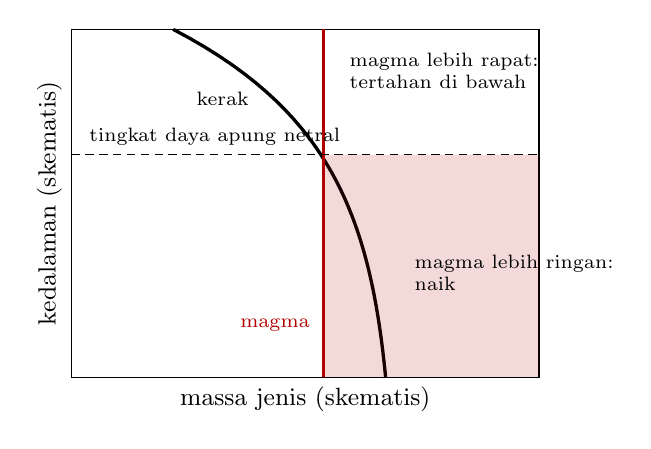
\begin{tikzpicture}[font=\scriptsize]
\begin{axis}[width=0.62\linewidth, height=6cm,
  xmin=0, xmax=1.15, ymin=0, ymax=1, y dir=reverse,
  xtick=\empty, ytick=\empty,
  xlabel={massa jenis (skematis)}, ylabel={kedalaman (skematis)},
  label style={font=\small}, clip=false]
\addplot[very thick, black, domain=0:1, samples=40] ({0.25 + 0.55*(1 - exp(-3*x))}, {x});
\addplot[very thick, red!70!black] coordinates {(0.62,0) (0.62,1)};
\fill[red!70!black, opacity=0.15] (axis cs:0.62,0.36) rectangle (axis cs:1.15,1);
\draw[densely dashed] (axis cs:0,0.36) -- (axis cs:1.15,0.36);
\node[anchor=south west] at (axis cs:0.02,0.36) {tingkat daya apung netral};
\node[anchor=east, black] at (axis cs:0.46,0.20) {kerak};
\node[anchor=east, red!70!black] at (axis cs:0.61,0.85) {magma};
\node[anchor=west, align=left] at (axis cs:0.82,0.70) {magma lebih ringan:\\naik};
\node[anchor=west, align=left] at (axis cs:0.66,0.12) {magma lebih rapat:\\tertahan di bawah};
\end{axis}
\end{tikzpicture}
\par\smallskip{\small \omterm{def:b2:magma-emplacement:ascent}{Tingkat daya apung netral} (skematis). Massa jenis
kerak bertambah terhadap kedalaman, karena pemadatan sedimen dan peralihan ke
batuan yang lebih rapat; \omterm{def:b2:magma-emplacement:magma}{magma} dengan massa jenis tetap naik selama lebih ringan daripada
sekelilingnya (diarsir) dan menyebar di tempat kedua massa jenis itu bertemu.}
\end{omfigure}

\omterm{def:b2:magma-emplacement:bodies}{Pluton} harus membuat ruang bagi dirinya. \omterm{def:b2:magma-emplacement:bodies}{Pluton} dapat mengangkat atapnya, seperti \omterm{def:b2:magma-emplacement:bodies}{lakolit};
\omterm{def:b2:magma-emplacement:bodies}{pluton} dapat mendesak dindingnya ke samping di tempat dinding itu lunak; \omterm{def:b2:magma-emplacement:bodies}{pluton} dapat mengisi ruang yang dibuka oleh
pensesaran; dan \omterm{def:b2:magma-emplacement:bodies}{pluton} dapat melakukan stoping pada atapnya, blok demi blok. \omterm{def:b2:magma-emplacement:bodies}{Pluton} besar lama
dibayangkan sebagai tangki \omterm{def:b2:magma-emplacement:magma}{magma} raksasa yang ditempatkan sekaligus. Penentuan umur telah mengubah
gambaran itu. Zirkon Tuolumne Intrusive Suite, sebuah \omterm{def:b2:magma-emplacement:bodies}{batolit} granit di
California, menunjukkan bahwa \omterm{def:b2:magma-emplacement:bodies}{batolit} itu ditempatkan antara \num{95} dan \qty{85}{Ma}, paling tua
di tepi dan paling muda di pusat, dan salah satu satuannya saja selama lebih
dari \qty{3}{Ma}, antara \qty{92.8}{Ma} dan \qty{88.8}{Ma}. Satu tubuh
\omterm{def:b2:magma-emplacement:magma}{magma} setebal \qty{5}{km} dan selebar \qty{20}{km} yang ditempatkan pada kedalaman \qty{15}{km} akan
mendingin di bawah \qty{750}{\celsius}, saat \omterm{def:b2:magma-emplacement:magma}{magma} itu kira-kira setengah terkristalkan, dalam
sekitar \num{500000}~tahun. \omterm{def:b2:magma-emplacement:bodies}{Pluton} semacam itu pasti dirakit secara bertahap,
dari banyak intrusi yang lebih kecil seperti lembaran dan \omterm{def:b2:magma-emplacement:bodies}{retas}, selama jutaan tahun
(\cref{exo:b2:magma-emplacement:11}).
% ledger: glazner04:tuolumne

\begin{omfigure}
\centering
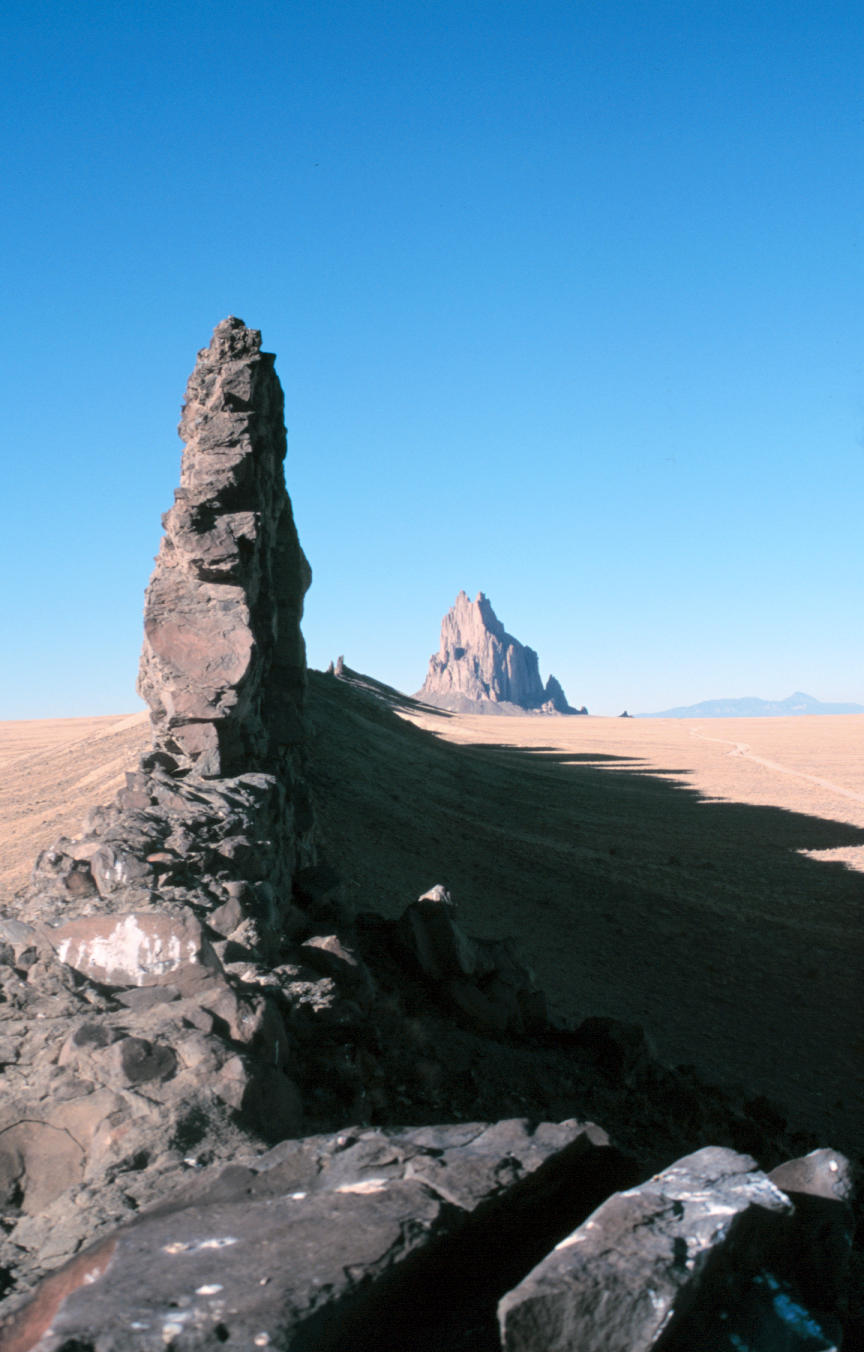
\includegraphics[width=0.3\linewidth]{images/book4/b2-shiprock-dyke.jpg}
\par\smallskip{\small Sebuah \omterm{def:b2:magma-emplacement:bodies}{retas} di dekat Shiprock, di Lapangan Vulkanik Navajo
(New Mexico): batuan \omterm{def:b2:magma-emplacement:bodies}{retas} lebih tahan erosi daripada batu pasir dan serpih
yang dipotongnya, dan kini berdiri sebagai tembok; di kejauhan, leher vulkanik yang menjadi pusat
beberapa \omterm{def:b2:magma-emplacement:bodies}{retas} semacam itu memancar. Foto: Dexter Perkins (CC0).}
\end{omfigure}

\section{Pendinginan dan metamorfisme kontak}

Intrusi kehilangan panasnya melalui konduksi ke batuan induknya. Model paling sederhana
memperlakukan intrusi dan batuan induknya sebagai satu medium penghantar dengan
difusivitas $\kappa$ yang seragam: pada waktu nol, lembaran setebal $b$ berada pada suhu
intrusi $T_m$ dan batuan induk pada $T_0$. Penyelesaian persamaan panas, dengan
$x$ diukur dari tengah lembaran, adalah
\[
T(x,t) = T_0 + \frac{T_m - T_0}{2}\left[\operatorname{erf}\frac{b/2 - x}{2\sqrt{\kappa t}}
+ \operatorname{erf}\frac{b/2 + x}{2\sqrt{\kappa t}}\right].
\]
Gambar di bawah menunjukkannya untuk \omterm{def:b2:magma-emplacement:bodies}{sill} setebal \qty{100}{m}.
% ledger: delaney86b4:properties

\begin{proposition}[Suhu kontak]\label{prop:b2:magma-emplacement:contact}
Dalam model ini, selama $\sqrt{\kappa t}$ kecil dibandingkan dengan $b$,
suhu pada kontak intrusi tetap pada rata-rata $(T_m + T_0)/2$
suhu intrusi dan suhu batuan induk.
\end{proposition}

\begin{proof}
Pada kontak $x = b/2$, fungsi galat pertama adalah $\operatorname{erf}0 = 0$ dan
yang kedua $\operatorname{erf}(b/(2\sqrt{\kappa t}))$, yang dekat dengan $1$ selama
$b \gg 2\sqrt{\kappa t}$. Maka $T = T_0 + (T_m - T_0)/2$.
\end{proof}

\omterm{def:b2:magma-emplacement:bodies}{Retas} basal pada \qty{1150}{\celsius} dalam batuan pada \qty{50}{\celsius} dengan demikian memanaskan
kontaknya hingga \qty{600}{\celsius}. Kalor kristalisasi, umumnya
\qtyrange{700}{1000}{MJ/m^3}, menjaga \omterm{def:b2:magma-emplacement:magma}{magma} tetap panas lebih lama dan menaikkan nilai ini:
dengan \qty{900}{MJ/m^3} yang dilepaskan antara \num{1150} dan \qty{950}{\celsius}, model yang sama
memberikan \qty{690}{\celsius}, sedangkan konduktivitas yang bergantung pada suhu dan batuan induk
yang basah menurunkan kedua taksiran itu sebesar 50 hingga \qty{75}{\celsius}.
% ledger: delaney86b4:dike, delaney86b4:properties

\begin{omfigure}
\centering
\begin{tikzpicture}
\begin{axis}[omrecord, width=0.86\linewidth, height=6cm,
  xmin=-200, xmax=200, ymin=0, ymax=1200,
  xlabel={jarak dari tengah sill (\unit{m})},
  ylabel={suhu (\unit{\celsius})},
  legend pos=north east, legend style={font=\scriptsize},
  tick label style={font=\scriptsize}, label style={font=\small}]
\fill[gray!15] (axis cs:-50,0) rectangle (axis cs:50,1200);
\addplot[very thick, red!80!black] table[x=x_m, y=t1] {figdata/out/bachelor-2-magma-sill.dat};
\addlegendentry{1 tahun}
\addplot[very thick, orange!90!black] table[x=x_m, y=t2] {figdata/out/bachelor-2-magma-sill.dat};
\addlegendentry{10 tahun}
\addplot[very thick, blue!60!black] table[x=x_m, y=t3] {figdata/out/bachelor-2-magma-sill.dat};
\addlegendentry{50 tahun}
\addplot[very thick, black] table[x=x_m, y=t4] {figdata/out/bachelor-2-magma-sill.dat};
\addlegendentry{200 tahun}
\draw[densely dashed, gray] (axis cs:-200,625) -- (axis cs:200,625);
\node[font=\scriptsize, gray!40!black, anchor=south west] at (axis cs:-198,625) {$(T_m + T_0)/2$};
\node[font=\scriptsize, anchor=south] at (axis cs:0,20) {sill};
\end{axis}
\end{tikzpicture}
\par\smallskip{\small Pendinginan konduktif \omterm{def:b2:magma-emplacement:bodies}{sill} setebal \qty{100}{m} (diarsir),
yang menerobos pada \qty{1150}{\celsius} ke dalam batuan bersuhu \qty{100}{\celsius}, dengan
$\kappa = \qty{0.7e-6}{m^2/s}$ dan tanpa kalor laten. Kontaknya tetap di sekitar
\qty{625}{\celsius} selama puluhan tahun sementara panas menyebar ke batuan induk; setelah dua
abad, \omterm{def:b2:magma-emplacement:bodies}{sill} dan sekelilingnya membentuk satu zona hangat yang lebar.}
\end{omfigure}
% ledger: delaney86b4:properties

Skala waktu pendinginan adalah waktu yang diperlukan panas untuk berdifusi melintasi
intrusi, berorde $(b/2)^2/\kappa$: sekitar \num{16} hari untuk \omterm{def:b2:magma-emplacement:bodies}{retas}
selebar \qty{2}{m}, satu abad untuk \omterm{def:b2:magma-emplacement:bodies}{sill} setebal \qty{100}{m}, seratus ribu tahun
untuk \omterm{def:b2:magma-emplacement:bodies}{pluton} berukuran beberapa kilometer. Kalor laten memperpanjangnya, demikian pula
keharusan membekukan \omterm{def:b2:magma-emplacement:magma}{magma}, bukan sekadar mendinginkannya.

\begin{proposition}[Pembekuan intrusi]\label{prop:b2:magma-emplacement:stefan}
Misalkan \omterm{def:b2:magma-emplacement:magma}{magma} pada suhu pembekuannya $T_m$, dengan kalor laten $L$ per satuan
volume, mengisi ruang $y > 0$ di samping batuan induk pada $T_0$ yang menempati $y < 0$, keduanya
dengan kapasitas kalor $\rho c$ per satuan volume dan difusivitas $\kappa$. Front
pembekuan maju sebagai $y_s = 2\lambda\sqrt{\kappa t}$, dengan $\lambda$
akar dari
\[
\frac{L\sqrt\pi}{\rho c\,(T_m - T_0)} = \frac{e^{-\lambda^2}}{\lambda\,(1 + \operatorname{erf}\lambda)},
\]
dan kontaknya tetap pada $T_0 + (T_m - T_0)/(1 + \operatorname{erf}\lambda)$. \omterm{def:b2:magma-emplacement:bodies}{Sill}
setebal $b$, yang membeku dari kedua dindingnya, menjadi padat setelah
$t = b^2/(16\lambda^2\kappa)$.
\end{proposition}

\begin{proof}
\omterm{def:b2:magma-emplacement:magma}{Magma} di depan front tetap pada $T_m$, sehingga panas hanya mengalir dalam padatan
dan batuan induk, tempat kita mencoba $T = T_0 + (T_m - T_0)(1 + \operatorname{erf}\xi)/(1 +
\operatorname{erf}\lambda)$ dengan $\xi = y/(2\sqrt{\kappa t})$. Setiap fungsi $\xi$
berbentuk $\alpha + \beta\operatorname{erf}\xi$ menyelesaikan persamaan panas; fungsi yang satu ini
mendekati $T_0$ jauh di dalam batuan induk ($\xi \to -\infty$) dan sama dengan $T_m$ pada front
$\xi = \lambda$. Pada $y = 0$ fungsi itu memberikan suhu kontak yang dinyatakan. Pada front,
kalor laten yang dilepaskan padatan yang maju, $L\,dy_s/dt = L\lambda\sqrt{\kappa/t}$
per satuan luas dan waktu, harus dihantarkan pergi, $k\,\partial T/\partial y = k(T_m -
T_0)\,e^{-\lambda^2}/[(1 + \operatorname{erf}\lambda)\sqrt{\pi\kappa t}]$. Menyamakan
keduanya dan memakai $k = \rho c\kappa$ menghasilkan persamaan untuk $\lambda$. Setiap dinding
\omterm{def:b2:magma-emplacement:bodies}{sill} menumbuhkan frontnya sendiri, secara independen selama intinya tetap pada $T_m$; kedua
front bertemu ketika $2\lambda\sqrt{\kappa t} = b/2$.
\end{proof}

Dengan kalor laten basal dan batuan induk bersuhu sekitar \qty{100}{\celsius},
$\lambda$ sekitar $0.65$: \omterm{def:b2:magma-emplacement:bodies}{sill} setebal \qty{100}{m} membeku dalam sekitar
tujuh puluh tahun, dan kontaknya tetap di sekitar \qty{740}{\celsius}, bukan
\qty{625}{\celsius}, selama proses itu. Soal akhir pekan menelusuri kasus ini.
Karena waktunya bertambah sebagai kuadrat ketebalan, \omterm{def:b2:magma-emplacement:bodies}{sill} yang sepuluh kali lebih tebal
memerlukan waktu seratus kali lebih lama.

\begin{definition}[Aureol kontak dan batuannya]\label{def:b2:magma-emplacement:aureole}
Yang disebut \emph{tepi dingin}\index{tepi dingin} adalah pinggiran intrusi yang berbutir halus atau bergelas,
tempat \omterm{def:b2:magma-emplacement:magma}{magma} mendingin dengan cepat terhadap batuan induk yang lebih dingin. Yang disebut
\emph{aureol kontak}\index{aureol kontak} adalah zona batuan induk di sekitar
intrusi yang termetamorfosis oleh panasnya. Yang disebut \emph{hornfels}\index{hornfels} adalah
batuan keras, berbutir halus, dan tidak berfoliasi yang terbentuk dari batu lumpur dan batuan vulkanik dalam
aureol kontak. Yang disebut \emph{skarn}\index{skarn} adalah batuan yang terbentuk ketika fluida magmatik
panas bereaksi dengan batuan induk karbonat, mengendapkan silikat kalsium--besi--magnesium
seperti garnet dan piroksen, sering bersama magnetit dan sulfida logam.
\end{definition}
% ledger: earle:intrusive-bodies, earle:skarn

\omterm{def:b2:magma-emplacement:aureole}{Aureol kontak} berkisar dari beberapa sentimeter di sekitar \omterm{def:b2:magma-emplacement:bodies}{retas} dan \omterm{def:b2:magma-emplacement:bodies}{sill} kecil hingga
beberapa puluh meter di sekitar stok yang besar, dan metamorfisme kontak mencakup
sekitar \qty{300}{\celsius} hingga lebih dari \qty{800}{\celsius}. Batu lumpur menjadi
\omterm{def:b2:magma-emplacement:aureole}{hornfels}, batu gamping menjadi marmer, batu pasir menjadi kuarsit. \omterm{def:b2:magma-emplacement:magma}{Magma} yang ditempatkan jauh
di dalam batuan yang sudah panas hampir tidak membuat aureol: lebarnya bergantung pada
ukuran dan suhu intrusi serta pada suhu batuan induknya, seperti
diramalkan model pendinginan (\cref{exo:b2:magma-emplacement:12}). Mineral yang tumbuh dalam aureol,
dan apa yang dikatakannya tentang suhu, termasuk dalam \cref{ch:b2:metamorphic-facies};
logam yang dipekatkan \omterm{def:b2:magma-emplacement:aureole}{skarn} termasuk dalam \cref{ch:b2:ore-deposits}.
% ledger: earle:skarn

\begin{inthefield}[Membaca kontak sebuah retas]
\begin{minipage}[t]{0.6\linewidth}\vspace{0pt}
Di tempat \omterm{def:b2:magma-emplacement:bodies}{retas} tersingkap, seorang ahli geologi pertama-tama menelusuri kontaknya dengan batuan
induk. Tepi yang lebih halus butirnya atau lebih bergelas daripada bagian tengah \omterm{def:b2:magma-emplacement:bodies}{retas} menunjukkan
bahwa \omterm{def:b2:magma-emplacement:magma}{magma} itu terdinginkan terhadap batuan yang dingin; sebuah \omterm{def:b2:magma-emplacement:bodies}{retas} selebar \qty{25}{cm} yang dipelajari
di pantai British Columbia memiliki \omterm{def:b2:magma-emplacement:aureole}{tepi dingin} setebal \qty{2}{cm}. Batuan
induk di samping kontak diamati untuk melihat tanda pemanggangan: perubahan warna, pengerasan,
mineral baru yang memudar menjauhi \omterm{def:b2:magma-emplacement:bodies}{retas}. Lebar zona terpanggang dan lebar
\omterm{def:b2:magma-emplacement:aureole}{tepi dingin}, yang dibandingkan dengan lebar \omterm{def:b2:magma-emplacement:bodies}{retas}, menunjukkan seberapa panas
batuan induk ketika \omterm{def:b2:magma-emplacement:bodies}{retas} itu datang; \omterm{def:b2:magma-emplacement:bodies}{retas} tanpa \omterm{def:b2:magma-emplacement:aureole}{tepi dingin} dan tanpa
aureol menerobos batuan yang sudah panas. Sampel diambil melintasi
\omterm{def:b2:magma-emplacement:bodies}{retas}, dari tepi ke tengah, untuk geokimia lelehannya dan untuk
ukuran kristalnya.
\end{minipage}\hfill
\begin{minipage}[t]{0.36\linewidth}\vspace{0pt}
\centering
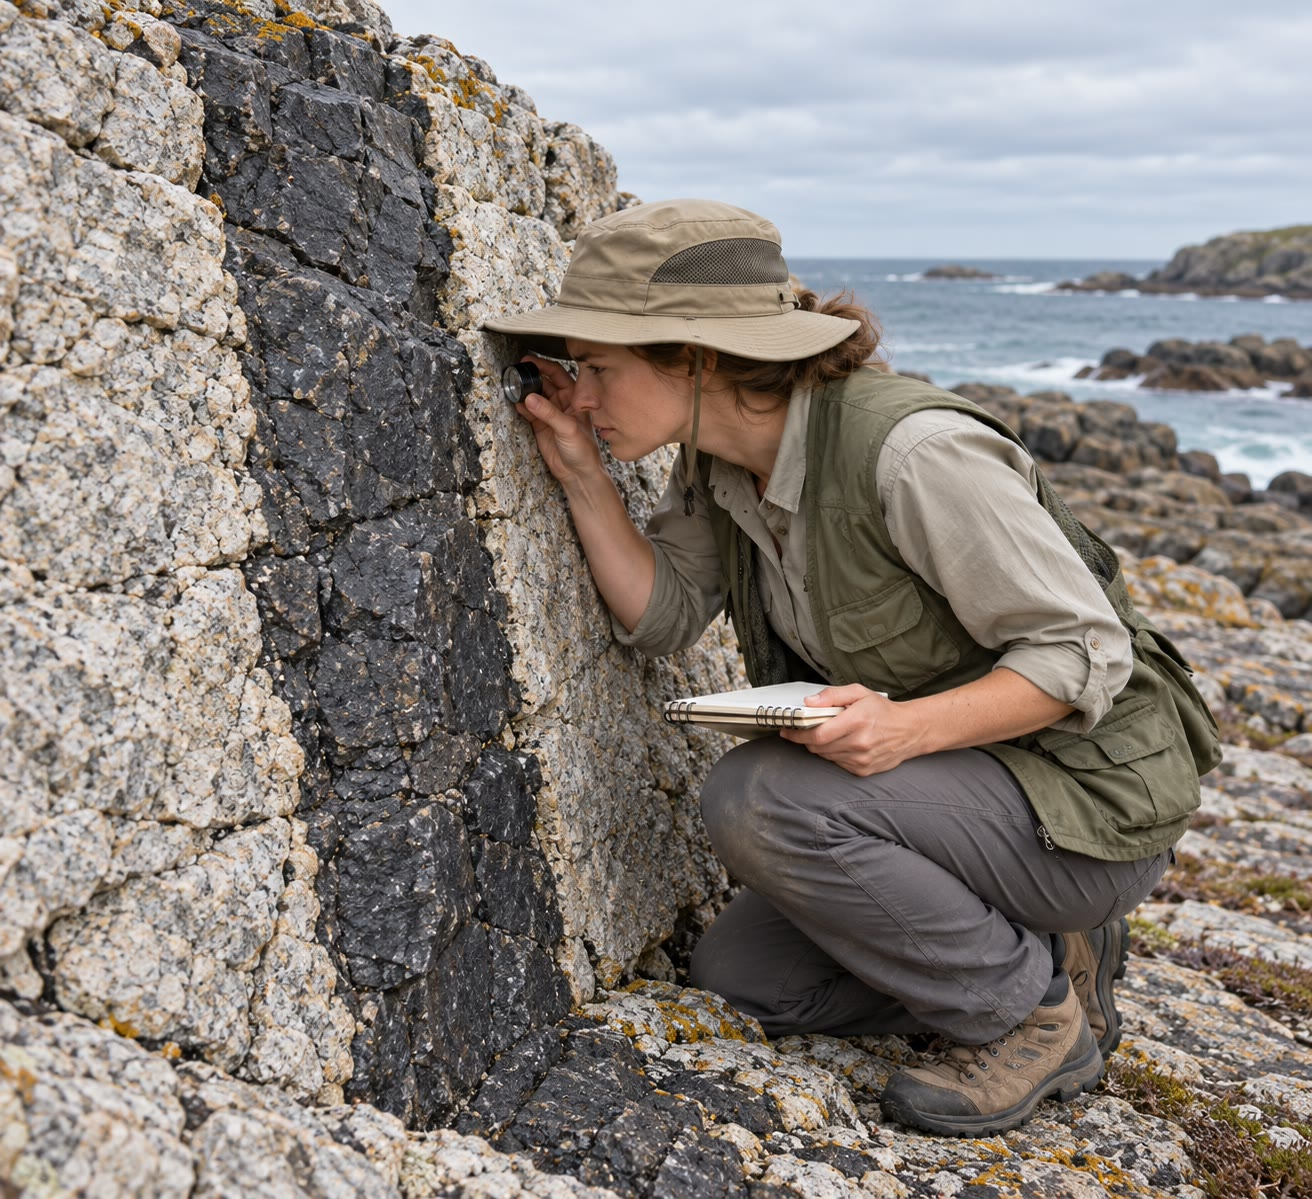
\includegraphics[width=\linewidth]{images/book4/ai/b2-dyke-contact.jpg}
\par\smallskip{\scriptsize Seorang ahli geologi mengamati kontak sebuah \omterm{def:b2:magma-emplacement:bodies}{retas} gelap dengan
batuan induk yang pucat (ilustrasi buatan AI).}
\end{minipage}
\end{inthefield}
% ledger: earle:intrusive-bodies

\section{Latihan}

\begin{exercise}[$\star$]\label{exo:b2:magma-emplacement:1}
Untuk lelehan granit yang mengandung air, sebuah persamaan yang dicocokkan dengan pengukuran memberikan
$\log_{10}\eta = [-3.545 + 0.833\ln w] + [9601 - 2368\ln w]/\{T - [195.7 + 32.25\ln
w]\}$, dengan $\eta$ dalam \unit{Pa.s}, $w$ kandungan air dalam persen berat, dan $T$
dalam kelvin. Hitunglah $\log_{10}\eta$ pada \qty{800}{\celsius} untuk $w = 1$ dan $w = 4$,
serta faktor penurunan viskositas oleh tiga persen air tambahan itu.
\end{exercise}
% ledger: hd96:model

\begin{exercise}[$\star$]\label{exo:b2:magma-emplacement:2}
Dengan hukum akar kuadrat, $s = 0.44$ untuk riolit dan $s = 0.34$ untuk basal
(persen berat per $\sqrt{\unit{MPa}}$), hitunglah tekanan jenuh
riolit dengan \qty{6}{\percent} air dan basal dengan \qty{0.5}{\percent},
serta kedalaman yang bersesuaian dalam kerak bermassa jenis \qty{2600}{kg/m^3}
($g = \qty{9.81}{m/s^2}$).
\end{exercise}

\begin{exercise}[$\star$]\label{exo:b2:magma-emplacement:3}
Hitunglah suhu kontak \omterm{def:b2:magma-emplacement:bodies}{retas} basal pada \qty{1150}{\celsius}
yang menerobos batuan pada \qty{50}{\celsius}, lalu batuan pada
\qty{400}{\celsius}. Manakah dari kedua \omterm{def:b2:magma-emplacement:bodies}{retas} itu yang akan memiliki \omterm{def:b2:magma-emplacement:aureole}{tepi dingin} yang lebih lebar?
\end{exercise}

\begin{exercise}[$\star$]\label{exo:b2:magma-emplacement:4}
Namailah setiap tubuh. (a) Lembaran dolerit setebal \qty{30}{m} yang terletak di antara dua lapisan
batu pasir sepanjang \qty{20}{km}. (b) Lembaran basal tegak selebar \qty{2}{m}
yang memotong batu gamping mendatar. (c) Granit yang tersingkap seluas \qty{2000}{km^2},
yang terdiri atas selusin satuan berumur berbeda. (d) Lensa porfiri selebar \qty{1}{km},
datar di dasarnya, yang di atasnya lapisan-lapisan melengkung ke atas. (e) Lembaran basal mendatar
di dalam granit.
\end{exercise}

\begin{exercise}[$\star\star$]\label{exo:b2:magma-emplacement:5}
Sebuah lelehan basal memiliki $\eta_{\ell} = \qty{100}{Pa.s}$. Dengan hubungan Einstein--Roscoe
($R = 1.35$), hitunglah viskositas \omterm{def:b2:magma-emplacement:magma}{magma} dengan
\qty{5}{\percent}, \qty{20}{\percent}, \qty{40}{\percent}, dan \qty{60}{\percent}
kristal, dan bandingkan yang pertama dengan rumus encer Einstein. Pada fraksi kristal
berapa hubungan itu meramalkan kemacetan?
\end{exercise}

\begin{exercise}[$\star\star$]\label{exo:b2:magma-emplacement:6}
\omterm{def:b2:magma-emplacement:magma}{Magma} yang massa jenisnya \qty{300}{kg/m^3} lebih kecil daripada dindingnya naik melalui \omterm{def:b2:magma-emplacement:bodies}{retas}.
(a) Untuk basal ($\eta = \qty{100}{Pa.s}$, $\rho = \qty{2700}{kg/m^3}$) dalam \omterm{def:b2:magma-emplacement:bodies}{retas}
selebar \qty{1}{m}, hitunglah kecepatan rata-rata, fluks per meter \omterm{def:b2:magma-emplacement:bodies}{retas},
bilangan Reynolds, dan waktu untuk naik \qty{10}{km}. (b) Waktu yang sama untuk riolit
\qty{e6}{Pa.s} dalam \omterm{def:b2:magma-emplacement:bodies}{retas} selebar \qty{1}{m}, lalu selebar \qty{10}{m}. (c) \omterm{def:b2:magma-emplacement:bodies}{Retas}
selebar \qty{1}{m} kehilangan panasnya dalam waktu berorde $(w/2)^2/\kappa$, dengan $\kappa =
\qty{1e-6}{m^2/s}$: manakah dari ketiga kenaikan itu yang dapat berhasil?
\end{exercise}

\begin{exercise}[$\star\star$]\label{exo:b2:magma-emplacement:7}
\omterm{def:b2:magma-emplacement:magma}{Magma} bermassa jenis \qty{2400}{kg/m^3} pada \qty{900}{\celsius} melepaskan
\qty{1}{\percent} massanya sebagai uap air. Dengan memperlakukan uap sebagai gas ideal
($R = \qty{8.314}{J/(mol.K)}$, \qty{18.015}{g/mol}), hitunglah fraksi volume
gas dalam \omterm{def:b2:magma-emplacement:magma}{magma} pada \qty{100}{MPa}, \qty{10}{MPa}, dan \qty{0.1}{MPa}. Manakah dari ketiga
nilai itu yang paling tidak dapat diandalkan, dan mengapa?
\end{exercise}

\begin{exercise}[$\star\star$]\label{exo:b2:magma-emplacement:8}
Dalam sebuah cekungan, massa jenis batuan bertambah terhadap kedalaman $z$ sebagai $\rho(z) =
2300 + 60\,z$ (\unit{kg/m^3}, $z$ dalam \unit{km}) hingga \qty{10}{km}. (a) Di mana
\omterm{def:b2:magma-emplacement:ascent}{tingkat daya apung netral} lelehan basal bermassa jenis \qty{2650}{kg/m^3}? (b) Model
massa jenis bab ini menunjukkan bahwa satu persen air terlarut menurunkan
massa jenis lelehan basal sekitar \qty{70}{kg/m^3}. Di mana lelehan dengan
satu persen air tambahan berhenti? (c) Berapa gaya apung per meter kubik
lelehan kering itu \qty{2}{km} di bawah \omterm{def:b2:magma-emplacement:ascent}{tingkat daya apung netralnya}?
\end{exercise}

\begin{exercise}[$\star\star$]\label{exo:b2:magma-emplacement:9}
Misalkan sebuah \omterm{def:b2:magma-emplacement:ascent}{diapir} granit berjari-jari \qty{1}{km} dengan defisit massa jenis
\qty{300}{kg/m^3} naik melalui kerak bawah dengan viskositas \qty{e19}{Pa.s}. Hitunglah
kecepatan Stokes-nya (bola kaku) dalam milimeter per tahun dan waktu untuk naik
\qty{10}{km}. Bandingkan dengan skala waktu $a^2/\kappa$ pendinginannya, dengan $\kappa
= \qty{1e-6}{m^2/s}$. Apa kesimpulanmu?
\end{exercise}

\begin{exercise}[$\star\star\star$]\label{exo:b2:magma-emplacement:10}
Air larut dalam lelehan baik sebagai molekul, $x_m = K_1 f$, maupun sebagai gugus
hidroksil, $x_{\mathrm{OH}}^2 = K_2 x_m$ (oksigen lelehan jauh berlebih), sehingga
air terlarut total adalah $x = x_m + x_{\mathrm{OH}}/2$. (a) Nyatakan $x$ sebagai
fungsi $f$ dan tunjukkan bahwa fungsi itu berperilaku sebagai $\sqrt f$ pada $f$ rendah dan sebagai $f$ pada
$f$ tinggi. (b) Pada fugasitas berapa kedua bentuk air sama melimpahnya? (c)
Dengan $K_1 = \qty{1e-4}{MPa^{-1}}$ dan $K_2 = 0.2$, hitunglah fugasitas itu, serta
bagian air yang larut sebagai hidroksil pada \qty{100}{MPa}.
\end{exercise}

\begin{exercise}[$\star\star\star$]\label{exo:b2:magma-emplacement:11}
Sebuah \omterm{def:b2:magma-emplacement:bodies}{pluton} granit sebesar \qty{1000}{km^3} dirakit selama \qty{4}{Ma}. (a) Hitunglah
pasokan \omterm{def:b2:magma-emplacement:magma}{magma} rata-ratanya dalam \unit{km^3} per tahun dan dalam \unit{m^3} per sekon. (b)
Satu \omterm{def:b2:magma-emplacement:bodies}{retas} sepanjang \qty{1}{km} dan selebar \qty{2}{m}, dengan kecepatan rata-rata
\qty{0.8}{m/s}, memasoknya: berapa lama \omterm{def:b2:magma-emplacement:bodies}{retas} itu akan mengantarkan seluruh
\omterm{def:b2:magma-emplacement:bodies}{pluton}? Berapa bagian dari \qty{4}{Ma} itu? (c) Jika \omterm{def:b2:magma-emplacement:bodies}{pluton} itu dibangun dari
lembaran setebal \qty{20}{m} dengan luas \qty{10}{km} kali \qty{10}{km}, berapa lembaran
yang diperlukan, dan berapa lama selang rata-rata antara dua lembaran? (d) Dengan
$\lambda = 0.65$ dan $\kappa = \qty{0.7e-6}{m^2/s}$, berapa lama sebuah lembaran
membeku? Apakah \omterm{def:b2:magma-emplacement:bodies}{pluton} itu pernah menjadi satu tubuh \omterm{def:b2:magma-emplacement:magma}{magma} yang besar?
\end{exercise}

\begin{exercise}[$\star\star\star$]\label{exo:b2:magma-emplacement:12}
Jauh dari \omterm{def:b2:magma-emplacement:bodies}{retas} tipis selebar $b$ (pada jarak $x \gg b$), panasnya bekerja sebagai
sumber bidang seketika: $T - T_0 = (T_m - T_0)\,b\,e^{-x^2/(4\kappa
t)}/\sqrt{4\pi\kappa t}$. (a) Tunjukkan bahwa pada jarak $x$ suhu paling tinggi pada
$t^* = x^2/(2\kappa)$, dan bahwa kenaikan tertinggi ini adalah $\Delta T_{\max} = (T_m -
T_0)\,b/(x\sqrt{2\pi e})$. (b) Untuk \omterm{def:b2:magma-emplacement:bodies}{retas} selebar \qty{2}{m} dengan $T_m - T_0 =
\qty{1100}{K}$, pada jarak berapa batuan menghangat paling banyak \qty{100}{K}, dan
kapan ($\kappa = \qty{0.7e-6}{m^2/s}$)? (c) Mengapa aureol \omterm{def:b2:magma-emplacement:bodies}{retas} tipis begitu
sempit?
\end{exercise}

\section{Soal: Sill di bawah plato}

\begin{problem}[{Soal akhir pekan --- mengikuti magma basal dari retas
pengumpannya hingga sebuah sill, airnya, dan waktu yang diperlukan sill untuk membeku}]
\label{pb:b2:magma-emplacement:1}
Di bawah sebuah plato khayalan, sedimen (serpih dan batu pasir) dengan massa jenis rata-rata
\qty{2450}{kg/m^3} terletak pada kedalaman \qty{3.0}{km} di atas batuan dasar kristalin dengan
massa jenis \qty{2800}{kg/m^3}. \omterm{def:b2:magma-emplacement:magma}{Magma} basal naik dari \qty{15}{km} melalui \omterm{def:b2:magma-emplacement:bodies}{retas}
selebar \qty{2.0}{m} dan menyebar di sepanjang dasar sedimen sebagai \omterm{def:b2:magma-emplacement:bodies}{sill} dolerit
setebal \qty{100}{m}. Data: suhu intrusi \qty{1150}{\celsius}; hukum viskositas
lelehan $\log_{10}\eta = -4.55 + 5510/(T - 611)$ ($T$ dalam kelvin); massa jenis
lelehan beserta airnya \qty{2710}{kg/m^3}; \qty{20}{\percent} kristal menurut volume
(Einstein--Roscoe, $R = 1.35$); air terlarut \qty{0.40}{\percent}, kelarutan
$s = 0.34$ persen per $\sqrt{\unit{MPa}}$; suhu batuan induk di tempat \omterm{def:b2:magma-emplacement:bodies}{sill}
\qty{100}{\celsius}; $\kappa = \qty{0.7e-6}{m^2/s}$, $\rho c = \qty{2.5}{MJ/(m^3.K)}$,
kalor laten \qty{900}{MJ/m^3}, dengan \omterm{def:b2:magma-emplacement:magma}{magma} dianggap membeku pada suhu
intrusinya; $g = \qty{9.81}{m/s^2}$; satu tahun adalah \qty{3.156e7}{s}.

\medskip\noindent\textbf{Bagian I --- Magmanya.}
\begin{enumerate}
\item Hitunglah $\log_{10}\eta$ dan $\eta$ lelehan pada \qty{1150}{\celsius}
(\qty{1423}{K}).
\item Hal yang sama pada \qty{1100}{\celsius}. Dengan faktor berapa viskositas berubah selama
\qty{50}{K} ini?
\item Hitunglah viskositas \omterm{def:b2:magma-emplacement:magma}{magma} beserta kristalnya pada
\qty{1150}{\celsius}.
\item Pada fraksi kristal berapa hubungan Einstein--Roscoe akan membuat
\omterm{def:b2:magma-emplacement:magma}{magma} macet? Bandingkan dengan taksiran lapangan tentang akhir aliran secara keseluruhan.
\item Hitunglah selisih massa jenis antara \omterm{def:b2:magma-emplacement:magma}{magma} dan batuan dasar, dan
antara \omterm{def:b2:magma-emplacement:magma}{magma} dan sedimen.
\item Hitunglah tekanan litostatik pada tingkat \omterm{def:b2:magma-emplacement:bodies}{sill}.
\end{enumerate}

\noindent\textbf{Bagian II --- Naik melalui retas.}
\begin{enumerate}[resume]
\item Hitunglah gradien tekanan apung $\Delta\rho\,g$ yang mendorong \omterm{def:b2:magma-emplacement:magma}{magma}
melalui batuan dasar.
\item Hitunglah kecepatan rata-rata \omterm{def:b2:magma-emplacement:magma}{magma} dalam \omterm{def:b2:magma-emplacement:bodies}{retas}.
\item Hitunglah fluks per meter \omterm{def:b2:magma-emplacement:bodies}{retas}, dan fluks totalnya jika \omterm{def:b2:magma-emplacement:bodies}{retas} itu
sepanjang \qty{1.0}{km}.
\item Hitunglah bilangan Reynolds aliran itu. Apakah alirannya laminar?
\item Berapa lama \omterm{def:b2:magma-emplacement:magma}{magma} naik dari \qty{15}{km} ke \qty{3.0}{km}?
\item Bandingkan dengan skala waktu $(w/2)^2/\kappa$ selama \omterm{def:b2:magma-emplacement:bodies}{retas} kehilangan
panasnya. Dapatkah \omterm{def:b2:magma-emplacement:bodies}{retas} itu tetap terbuka?
\item Jelaskan mengapa \omterm{def:b2:magma-emplacement:magma}{magma} berhenti pada \qty{3.0}{km} dan menyebar ke samping, dengan
kosakata bab ini.
\end{enumerate}

\noindent\textbf{Bagian III --- Airnya.}
\begin{enumerate}[resume]
\item Hitunglah tekanan jenuh air lelehan, dan kedalaman di dalam
sedimen tempat tekanan itu tercapai.
\item Berapa banyak air yang dapat ditampung lelehan pada tingkat \omterm{def:b2:magma-emplacement:bodies}{sill}? Apakah \omterm{def:b2:magma-emplacement:magma}{magma} \omterm{def:b2:magma-emplacement:bodies}{sill}
itu melakukan eksolusi air?
\item Vesikel di \omterm{def:b2:magma-emplacement:aureole}{tepi dingin} \omterm{def:b2:magma-emplacement:bodies}{sill} sebagian besar berisi CO$_2$. Jelaskan.
\item Jika seluruh \qty{0.40}{\percent} air keluar di permukaan, pada
\qty{1150}{\celsius} dan \qty{0.1}{MPa}, berapa fraksi volume \omterm{def:b2:magma-emplacement:magma}{magma} yang akan
ditempati uap itu (gas ideal)?
\end{enumerate}

\noindent\textbf{Bagian IV --- Pendinginan dan pembekuan.}
\begin{enumerate}[resume]
\item Dengan mengabaikan kalor laten, hitunglah suhu kontak \omterm{def:b2:magma-emplacement:bodies}{sill}.
\item Dengan mengabaikan kalor laten, hitunglah suhu \qty{10}{m} di atas kontak
atas \num{10}~tahun setelah intrusi.
\item Model yang sama: hitunglah suhu di tengah \omterm{def:b2:magma-emplacement:bodies}{sill} setelah
\num{10}~tahun dan \num{50}~tahun.
\item Model yang sama: \qty{80}{m} di atas kontak atas, hitunglah suhu setelah
\num{300}, \num{363}, dan \num{420} tahun. Apakah batuan di sana pernah mencapai
\qty{300}{\celsius}?
\item Hitunglah $L\sqrt\pi/(\rho c\,(T_m - T_0))$ untuk \omterm{def:b2:magma-emplacement:bodies}{sill} itu.
\item Evaluasilah $e^{-\lambda^2}/(\lambda(1 + \operatorname{erf}\lambda))$ untuk $\lambda = 0.64$,
$0.65$, dan $0.66$ ($\operatorname{erf}0.64 = 0.6346$, $\operatorname{erf}0.65 = 0.6420$,
$\operatorname{erf}0.66 = 0.6494$), dan berikan $\lambda$ hingga dua desimal.
\item Dengan kalor laten, hitunglah suhu kontak selama \omterm{def:b2:magma-emplacement:bodies}{sill}
membeku. Mengapa suhu itu lebih tinggi daripada pada pertanyaan 18?
\item Hitunglah skala waktu $(b/2)^2/\kappa$ dalam tahun.
\item Hitunglah waktu yang diperlukan \omterm{def:b2:magma-emplacement:bodies}{sill} untuk membeku, dalam tahun, yaitu angka kunci
soal ini, dan jelaskan mengapa waktu itu lebih pendek daripada skala waktu pada pertanyaan
terakhir meskipun kalor laten harus dikeluarkan.
\end{enumerate}
\end{problem}
% ledger: grd08:model, kolz22:einstein-roscoe, glazner04:tuolumne, moore98:h2o, lowenstern01:co2, delaney86b4:properties
